%TODOS FOR THIS LAB
%1.  Maybe merge mst and ImgSegMST
% Note: Prim's section has been taken out since it was covered in class, content is commented out
% Kruskal's section also contains a short comparison of Kruskal's and Prim's

\lab{Kruskal's Algorithm}{Kruskal's Algorithm}

\label{lab:Kruskal}

\objective{Find a minimum spanning tree for a connected, weighted graph using Kruskal's Algorithm}

\section*{Weighted Graphs and Spanning trees}

In this lab we will focus on graphs that are \emph{connected, undirected}, and \emph{weighted}. Recall that a graph is represented as a set of nodes combined with a set of edges that connect the nodes. A \emph{connected graph} is a graph where there is a path between each pair of nodes. If the directions of these edges are specified, we have a \emph{directed graph}, and if all of the edges are bidirectional, we have an \emph{undirected graph}.

\begin{figure}[h]
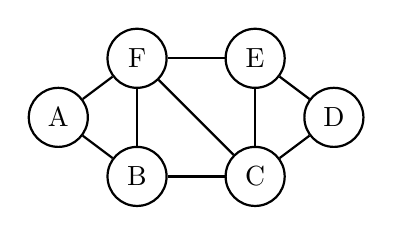
\begin{tikzpicture}[node distance= 1.5cm, thick, main 
	node/.style={circle, draw, minimum size = .75cm}]

\node[main node](B)[]{B};
\node[main node](C)[right of=B]{C};
\node[main node](F)[above of=B]{F};
\node[main node](E)[right of=F]{E};
\node[draw=none, node distance=.75cm](dummy)[above of= B]{};
\node[main node, node distance=1cm](A)[left of=dummy]{A};
\node[main node, node distance=2.5cm](D)[right of=dummy]{D};

\foreach \s/\t in {A/B, B/F, F/C, B/C, F/E, E/D, C/D, E/C, A/F}{\path[draw] (\s) edge (\t);}

\end{tikzpicture}
\caption{An example of a connected, undirected graph}
\label{mst:graph1}
\end{figure}

A \emph{weighted graph} is a graph where each edge has a value associated with it.
Usually these values represent some sort of cost or distance. For example, if we had a graph representing cities in the U.S., the weights between nodes (cities) would be the distance between the two cities. We represent the graph in the figure above as an adjacency matrix. Note that since the graph is undirected, the matrix is symmetric.

\[
\bordermatrix{\hspace{.4cm}&A&B&C&D&E&F\cr
A&0 & 1 & 0 & 0 & 0 & 1\cr
B&1 & 0 & 1 & 0 & 0 & 1\cr
C&0 & 1 & 0 & 1 & 1 & 1\cr
D&0 & 0 & 1 & 0 & 1 & 0\cr
E&0 & 0 & 1 & 1 & 0 & 1\cr
F&1 & 1 & 1 & 0 & 1 & 0\cr}
\]

Now consider the graph in Figure \ref{mst:graph4}.  This graph is the same as the graph in Figure \ref{mst:graph1}, except now there is a weight attached to each edge.  The adjacency matrix for this graph is
\[
\bordermatrix{\hspace{.4cm}&A&B&C&D&E&F\cr
A&0 & 3 & 0 & 0 & 0 & 6\cr
B&3 & 0 & 5 & 0 & 0 & 4\cr
C&0 & 5 & 0 & 1 & 1 & 5\cr
D&0 & 0 & 1 & 0 & 2 & 0\cr
E&0 & 0 & 1 & 2 & 0 & 4\cr
F&6 & 4 & 5 & 0 & 4 & 0\cr}
\]

We can also represent weighted graphs as adjacency lists. When we make the adjacency list of a directed, unweighted graph, we can make a dictionary with each node as a key and a list of its neighbors as the corresponding value. We can also make a list of the pairs of nodes corresponding to each edge (we will need two pairs to represent each edge in an undirected graph). For a weighted graph, we add a third value representing the weight of that edge.
Such a list for our undirected, weighted graph would look like the following:

\begin{lstlisting}
[('A', 'F', 6), ('A', 'B', 3), ('B', 'A', 3), ('B', 'C', 5), ('B', 'F', 4),
 ('C', 'B', 5), ('C', 'D', 1), ('C', 'E', 1), ('C', 'F', 5), ('D', 'C', 1), 
 ('D', 'E', 2), ('E', 'C', 1), ('E', 'D', 2), ('E', 'F', 4), ('F', 'A', 6), 
 ('F', 'B', 4), ('F', 'C', 5), ('F', 'E', 4)]
\end{lstlisting}

A \emph{spanning tree} of a connected, undirected graph $G$ is an undirected graph that contains all the nodes of $G$, a subset of the edges, and no cycles.
A cycle, for undirected graphs, is a path where you start and end on the same node without crossing any edge more than once.
The red in Figure \ref{mst:graph2} is an example of a cycle in an undirected graph.

\begin{figure}[H]
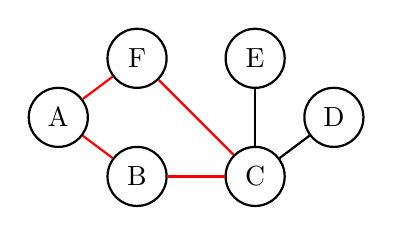
\begin{tikzpicture}[node distance= 1.5cm, thick, main 
	node/.style={circle, draw, minimum size = .75cm}]

\node[main node](B)[]{B};
\node[main node](C)[right of=B]{C};
\node[main node](F)[above of=B]{F};
\node[main node](E)[right of=F]{E};
\node[draw=none, node distance=.75cm](dummy)[above of= B]{};
\node[main node, node distance=1cm](A)[left of=dummy]{A};
\node[main node, node distance=2.5cm](D)[right of=dummy]{D};

\foreach \s/\t in {A/B, A/F, F/C, B/C}{\path[draw, red](\s) edge (\t);}
\foreach \s/\t in {E/C, C/D}{\path[draw](\s)edge(\t);} 

\end{tikzpicture}
\caption{A cycle in an undirected graph.}
\label{mst:graph2}
\end{figure}

The minimum spanning tree (MST) of a weighted, undirected graph is a spanning tree where the total weight is less than or equal to the total weight of every other spanning tree.
Kruskal's Algorithm is a method that finds the minimum spanning tree of a weighted, undirected graph.
Figure \ref{mst:graph3} shows a spanning tree of the graph shown in Figure \ref{mst:graph1}.
Figure \ref{mst:graph5} shows a minimum spanning tree of the graph shown in Figure \ref{mst:graph4}.

\begin{figure}[H]
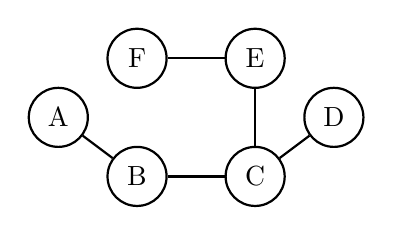
\begin{tikzpicture}[node distance= 1.5cm, thick, main 
	node/.style={circle, draw, minimum size = .75cm}]

\node[main node](B)[]{B};
\node[main node](C)[right of=B]{C};
\node[main node](F)[above of=B]{F};
\node[main node](E)[right of=F]{E};
\node[draw=none, node distance=.75cm](dummy)[above of= B]{};
\node[main node, node distance=1cm](A)[left of=dummy]{A};
\node[main node, node distance=2.5cm](D)[right of=dummy]{D};

\foreach \s/\t in {A/B, B/C, F/E, E/C, C/D}{\path[draw](\s)edge(\t);}
\end{tikzpicture}
\caption{A spanning tree with no cycles for the graph in Figure \ref{mst:graph1}.}
\label{mst:graph3}
\end{figure}



\begin{figure}[H]
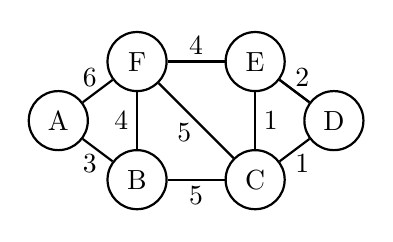
\begin{tikzpicture}[node distance= 1.5cm, thick, main 
	node/.style={circle, draw, minimum size = .75cm}]

\node[main node](B)[]{B};
\node[main node](C)[right of=B]{C};
\node[main node](F)[above of=B]{F};
\node[main node](E)[right of=F]{E};
\node[draw=none, node distance=.75cm](dummy)[above of= B]{};
\node[main node, node distance=1cm](A)[left of=dummy]{A};
\node[main node, node distance=2.5cm](D)[right of=dummy]{D};

\node[draw=none]at (-.6,.2)(3){3};
\node[draw=none]at (-.2,.75)(4){4};
\node[draw=none]at (.75,1.7)(4_2){4};
\node[draw=none]at (1.7,.75)(1){1};
\node[draw=none]at (2.1,.2)(1_2){1};
\node[draw=none]at (-.6,1.3)(6){6};
\node[draw=none]at (.75, -.2)(5){5};
\node[draw=none]at (2.1,1.3)(2){2};
\node[draw=none]at (.6,.6)(five){5};

\foreach \s/\t in {A/B, B/F, F/C, B/C, F/E, E/D, C/D, E/C, A/F, E/D}{\path[draw] (\s) edge (\t);}

\end{tikzpicture}
\caption{A weighted, undirected graph}
\label{mst:graph4}
\end{figure}

\begin{figure}[H]
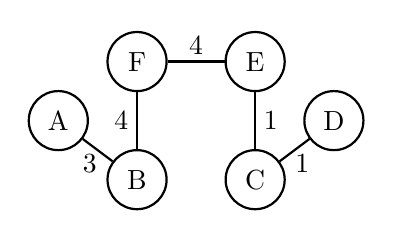
\begin{tikzpicture}[node distance= 1.5cm, thick, main 
	node/.style={circle, draw, minimum size = .75cm}]

\node[main node](B)[]{B};
\node[main node](C)[right of=B]{C};
\node[main node](F)[above of=B]{F};
\node[main node](E)[right of=F]{E};
\node[draw=none, node distance=.75cm](dummy)[above of= B]{};
\node[main node, node distance=1cm](A)[left of=dummy]{A};
\node[main node, node distance=2.5cm](D)[right of=dummy]{D};

\foreach \s/\t in {A/B, B/F, F/E, E/C, C/D}{\path[draw](\s)edge(\t);}
\node[draw=none]at (-.6,.2)(3){3};
\node[draw=none]at (-.2,.75)(4){4};
\node[draw=none]at (.75,1.7)(4_2){4};
\node[draw=none]at (1.7,.75)(1){1};
\node[draw=none]at (2.1,.2)(1_2){1};

\end{tikzpicture}
\caption{The MST of the graph in Figure \ref{mst:graph4}.}
\label{mst:graph5}
\end{figure}

\section*{Kruskal's algorithm}

Given a connected, weighted graph G with $n$ nodes, Kruskal's algorithm finds a minimum spanning tree. It is similar to Prim's algorithm, which also finds a minimum spanning tree of a connected, weighted graph. While Prim's algorithm is much faster for dense graphs since it avoids sorting the edges, it is much slower than Kruskal's for sparse graphs. Note that although we have not explicitly required that the graph be undirected, the fact that we are finding a minimum spanning tree means that the graph must be undirected.

Kruskal's algorithm first sorts the edges from smallest to largest, then starting with the smallest, the algorithm adds edges to the tree as long as the addition of each new edge does not create a cycle.
When $n-1$ edges have been added, the algorithm stops.

In order to avoid creating cycles while building the tree, it is necessary to keep track of which portions of the tree currently lie in connected groups.
This can be done by creating a dictionary where, when the algorithm starts, each node points to itself as the root of its own tree.
As we iterate over the edges, we compare the roots of the nodes connected by the edge. If they are distinct, then the nodes are in separate trees, so adding this edge will not create a cycle. When we add an edge, we update the root of one of the nodes connected by it so we can track which nodes are already connected by our growing MST.
We apply Kruskal's algorithm to the graph in Figure \ref{mst:graph4}. We are given a list of edges. Note that since the graph is undirected, we only have one entry for each edge instead of including both \li{(A, B, 2)} and \li{(B, A, 2)} for an edge from \li{A} to \li{B} with weight 2. Before beginning, we initialize what will become our MST as an empty list, initialize a dictionary \li{\{A:A, B:B, C:C, D:D, E:E, F:F\}} where each node points to itself, and sort the edges by weight to get the list \li{[(C, D, 1), (C, E, 1), (D, E, 2), (A, B, 3), (B, F, 4), (E, F, 4), (B, C, 5), (C, F, 5), (A, F, 6)]}. Since there are six nodes in the graph, we will continue until we have 5 edges in the tree.

\vspace{.25cm}

\begin{minipage}{0.35\textwidth}
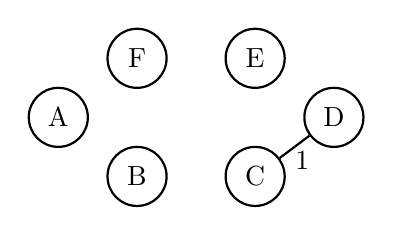
\begin{tikzpicture}[node distance= 1.5cm, thick, main 
	node/.style={circle, draw, minimum size = .75cm}]

\node[main node](B)[]{B};
\node[main node](C)[right of=B]{C};
\node[main node](F)[above of=B]{F};
\node[main node](E)[right of=F]{E};
\node[draw=none, node distance=.75cm](dummy)[above of= B]{};
\node[main node, node distance=1cm](A)[left of=dummy]{A};
\node[main node, node distance=2.5cm](D)[right of=dummy]{D};

\foreach \s/\t in {C/D}{\path[draw](\s)edge(\t);}
%\node[draw=none]at (1.7,.75)(1){1};
\node[draw=none]at (2.1,.2)(1_2){1};

\end{tikzpicture}
\end{minipage}\hfill
\begin{minipage}{0.55\textwidth}
We begin iterating through the edges to build the tree.
The first edge in the list is \li{(C,D,1)}.
The root for \li{C} is \li{C} and the root for \li{D} is \li{D}. Since their roots are distinct, they are in separate trees, so we add this edge to the tree. The tree becomes \li{[(C, D, 1)]}.
We then change the root node of \li{D} to \li{C}.
The dictionary of root nodes is now \li{\{A:A, B:B, C:C, D:C, E:E, F:F\}}.
\end{minipage}

\vspace{.25cm}

\begin{minipage}{0.35\textwidth}
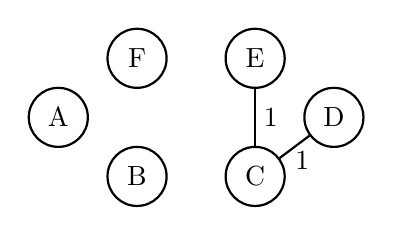
\begin{tikzpicture}[node distance= 1.5cm, thick, main 
	node/.style={circle, draw, minimum size = .75cm}]

\node[main node](B)[]{B};
\node[main node](C)[right of=B]{C};
\node[main node](F)[above of=B]{F};
\node[main node](E)[right of=F]{E};
\node[draw=none, node distance=.75cm](dummy)[above of= B]{};
\node[main node, node distance=1cm](A)[left of=dummy]{A};
\node[main node, node distance=2.5cm](D)[right of=dummy]{D};

\foreach \s/\t in {C/D, C/E}{\path[draw](\s)edge(\t);}
\node[draw=none]at (1.7,.75)(1){1};
\node[draw=none]at (2.1,.2)(1_2){1};

\end{tikzpicture}
\end{minipage}\hfill
\begin{minipage}{0.55\textwidth}
Now we process the next edge, \li{(C, E, 1)}.
The root node of \li{C} is \li{C}, and the root node of \li{E} is \li{E}, so adding this edge does not create a cycle.
We add this edge into the tree, so the tree is now \li{[(C, D, 1), (C, E, 1)]}.
Then we change the root of \li{E} to \li{C}, so the dictionary is \li{\{A:A, B:B, C:C, D:C, E:C, F:F\}}.
\end{minipage}

\vspace{.25cm}

The next edge is \li{(D, E, 2)}.
The root node of the tree containing \li{D} is \li{C} and the root node of the tree containing \li{E} is \li{C}, so these nodes are already connected, so we do not add this edge to the tree.

\vspace{.25cm}

\begin{minipage}{0.35\textwidth}
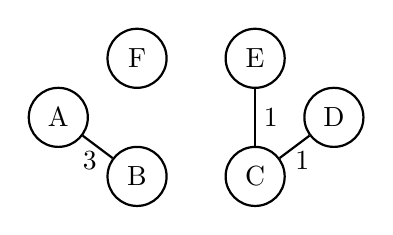
\begin{tikzpicture}[node distance= 1.5cm, thick, main 
	node/.style={circle, draw, minimum size = .75cm}]

\node[main node](B)[]{B};
\node[main node](C)[right of=B]{C};
\node[main node](F)[above of=B]{F};
\node[main node](E)[right of=F]{E};
\node[draw=none, node distance=.75cm](dummy)[above of= B]{};
\node[main node, node distance=1cm](A)[left of=dummy]{A};
\node[main node, node distance=2.5cm](D)[right of=dummy]{D};

\foreach \s/\t in {A/B, E/C, C/D}{\path[draw](\s)edge(\t);}
\node[draw=none]at (-.6,.2)(3){3};
\node[draw=none]at (1.7,.75)(1){1};
\node[draw=none]at (2.1,.2)(1_2){1};

\end{tikzpicture}
\end{minipage}\hfill
\begin{minipage}{0.55\textwidth}
The next edge is \li{(A, B, 3)}.
The root node for \li{A} is \li{A}, and the root node for \li{B} is \li{B}, so we add the edge to the tree and change the root node of \li{B} to \li{A}.
The dictionary becomes \li{\{A:A, B:A, C:C, D:C, E:C, F:F\}}
\end{minipage}\hfill

\vspace{.25cm}

\begin{minipage}{0.35\textwidth}
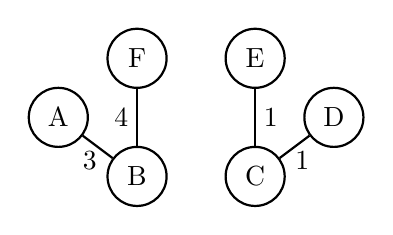
\begin{tikzpicture}[node distance= 1.5cm, thick, main 
	node/.style={circle, draw, minimum size = .75cm}]

\node[main node](B)[]{B};
\node[main node](C)[right of=B]{C};
\node[main node](F)[above of=B]{F};
\node[main node](E)[right of=F]{E};
\node[draw=none, node distance=.75cm](dummy)[above of= B]{};
\node[main node, node distance=1cm](A)[left of=dummy]{A};
\node[main node, node distance=2.5cm](D)[right of=dummy]{D};

\foreach \s/\t in {A/B, B/F, E/C, C/D}{\path[draw](\s)edge(\t);}
\node[draw=none]at (-.6,.2)(3){3};
\node[draw=none]at (-.2,.75)(4){4};
%\node[draw=none]at (.75,1.7)(4_2){4};
\node[draw=none]at (1.7,.75)(1){1};
\node[draw=none]at (2.1,.2)(1_2){1};

\end{tikzpicture}
\end{minipage}\hfill
\begin{minipage}{0.55\textwidth}
The next edge is \li{(B, F, 4)}.
The root node for \li{B} is \li{A} and the root node for \li{F} is \li{F}, so we add the edge to the tree and change the root node of \li{F} to \li{A}.
The dictionary becomes \li{\{A:A, B:A, C:C, D:C, E:C, F:A\}}
\end{minipage}\hfill

\vspace{.25cm}

\begin{minipage}{0.35\textwidth}
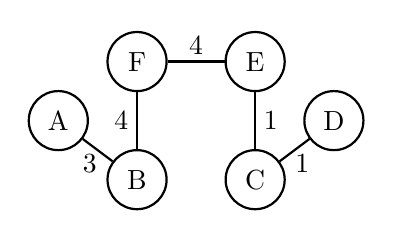
\begin{tikzpicture}[node distance= 1.5cm, thick, main 
	node/.style={circle, draw, minimum size = .75cm}]

\node[main node](B)[]{B};
\node[main node](C)[right of=B]{C};
\node[main node](F)[above of=B]{F};
\node[main node](E)[right of=F]{E};
\node[draw=none, node distance=.75cm](dummy)[above of= B]{};
\node[main node, node distance=1cm](A)[left of=dummy]{A};
\node[main node, node distance=2.5cm](D)[right of=dummy]{D};

\foreach \s/\t in {A/B, B/F, F/E, E/C, C/D}{\path[draw](\s)edge(\t);}
\node[draw=none]at (-.6,.2)(3){3};
\node[draw=none]at (-.2,.75)(4){4};
\node[draw=none]at (.75,1.7)(4_2){4};
\node[draw=none]at (1.7,.75)(1){1};
\node[draw=none]at (2.1,.2)(1_2){1};

\end{tikzpicture}
\end{minipage}\hfill
\begin{minipage}{0.55\textwidth}
The next edge is \li{(E, F, 4)}.
The root node for \li{E} is \li{C} and the root node for \li{F} is \li{A}.
We add the edge to the tree and end the algorithm since there are now 5 edges in the tree.
(If we were to continue the algorithm, we would change the root node of \li{A} to \li{C}.)
\end{minipage}

\vspace{.25cm}

Notice how we updated the root of the root node to one of the nodes in the edge added.
We manage the root nodes in this manner in order to find the root node by tracing back through the dictionary until we find a node that points to itself.
For example, to find the root node of \li{F} we first need to get the value for \li{F} from the dictionary.  This is \li{A}.
Then we get the value for \li{A} from the dictionary which is \li{C}.
Since the value of \li{C} in the dictionary is itself, the \li{C} is the root node of the graph containing \li{F}.
It is necessary to trace through the dictionary in this manner each time because it allows us to avoid iterating over all of the nodes and updating their root values everytime.


Algorithm \ref{alg:kruskal} outlines the psuedocode for the algorithm as described above:
\begin{algorithm}
\begin{algorithmic}[1]
\Procedure{kruskal}{$edges$}
	\State $tree \gets \text{Empty list of edges for MST}$
	\State $nodes \gets \text{Dictionary that points each node towards its root, initially itself}$
	\State $remaining \gets \text{Set number of nodes to be processed to } n-1$
	\Function{track}{$node$} \Comment{Find the root of the given node}
		\State $temp \gets \text{Node whose root we are finding}$
		\While{$temp$ does not point to itself in the dictionary}
			\State Update $temp$ to be the node it currently points to in $nodes$
			\State \pseudoli{return} $temp$
		\EndWhile
	\EndFunction
	\For{$n_1, n_2, weight$ in sorted list of edges}
		\State $root \gets \text{Root node of } n_1$
		\State $remove \gets \text{Root node of } n_2$
		\If{$root$ is not $remove$}
			\State Add the edge to the tree
			\State Lower $remaining$ by 1
			\If{$remaining$ is 0}
				\State \pseudoli{return} $tree$
			\EndIf
			\State Change the value associated with $remove$ to $root$
		\EndIf
	\EndFor	
\EndProcedure
\end{algorithmic}
\caption{Kruskal's algorithm for finding a MST}
\label{alg:kruskal}
\end{algorithm}

\begin{comment}
Previous description of the algorithm
\begin{itemize}

% Note: The comments in the solutions match the pseudocode.
% When making changes, please keep that in mind.

\item Initialize an empty list of edges for the minimum spanning tree.

\item Make a dictionary that points each node toward its root (not always directly to it).
Start with each node pointing to itself.

\item Initialize the number of nodes that still need to be processed to the number of nodes minus 1.

\item Define a helper function that, given a node, traces through the dictionary to find the root of its tree.
This can be done like this:

	\begin{itemize}

	\item Initialize a temporary variable to be the node for which we are finding the root.

	\item While the temporary node does not point to itself in the dictionary:

		\begin{itemize}

		\item Update the temporary node to be the node it currently points to in the dictionary.

		\end{itemize}

	\item Return the temporary node.

	\end{itemize}

\item Iterate over the edges by ascending weight.
Use a \li{for} loop for this and return the tree when it is big enough which breaks the loop for you.

	\begin{itemize}

	\item Trace through the dictionary to find the root node of each of the nodes in the edge you are processing.

	\item If the roots are not the same (i.e. if adding the edge doesn't form a cycle):

		\begin{itemize}

		\item Add the edge to the tree.

		\item Lower the number of edges remaining by one.

		\item If the number of edges remaining is 0, return the tree (which also breaks the loop).

		\item Update the root of the root of the second node in the edge to be the root of the first node in the edge.
			This lets us record that the two subtrees are now connected.

		\end{itemize}

	\end{itemize}

\end{itemize}
\end{comment}
Notice that if $remaining$ is 0, that means that the MST is as big as it needs to be and the for loop ends, and that updating the root of the second node in the edge is what allows us to check if two nodes are already connected.

You can iterate over a sorted copy of a list using the built in \li{sorted} function.
You can sort by the third value in each tuple using the \li{itemgetter} function that is part of the \li{operator} library included with Python.
For example:
\begin{lstlisting}
from operator import itemgetter

for n1, n2, weight in sorted(edges, key=itemgetter(2)):
    ...
\end{lstlisting}

\begin{problem}
Implement Kruskal's algorithm as in Algorithm \ref{alg:kruskal}
Test your algorithm on lists of weighted edges generated by the \li{randgraph} function below. Also use the data from MSTdata.npy to test your algorithm.
Use np.load("MSTdata.npy") to get it, and use the \li{formChanger} function below to put it in the right form.
\begin{lstlisting}
from scipy import linalg as la
import numpy as np

# n is the number of nodes in the graph
def randgraph(n):
    # Creates a sparse upper triangular matrix of ints between 1 and 50
    A = la.triu(np.random.randint(1,50,(n,n))*(np.random.rand(n,n)>.5))
    S = []
    # Iterate through (i,j) pairs in A; x is the value of (i,j)
    for index, x in np.ndenumerate(A):
        # If an edge exists
        if x != 0:
            # Append (i,j) as an edge with weight x
            S.append((str(index[0]), str(index[1]), x))

def formChanger(oldData):
    newData=[]
    for i in oldData: newData.append((i[0],i[1],int(i[2])))
    return newData
\end{lstlisting}
\end{problem}

\begin{comment}
\section*{Prim's algorithm}

Prim's is a similar algorithm for finding minimum spanning trees.
While it is much slower than Kruskal's algorithm for sparse graphs, it is much faster for dense graphs because Prim's algorithm avoids sorting the edges.

Again, consider the example shown in Figure 7.4.
We first initialize a dictionary with all the nodes as keys in order to track which nodes have not been processed.
At the beginning it will be \li{\{A:False, B:False, C:False, D:False, E:False, F:False\}}.
We then form the dictionary that maps each node to the edges that contain it.
Since we will already know one node of each edge while we use the dictionary, we only need to store the node that is not being looked up.
It should end up looking like \li{\{A:[(B, 3), (F, 6)], B:[(A, 3), (C, 5), (F, 4)], C:[(B, 5), (D, 1), (E, 1), (F, 5)], D:[(C, 1), (E, 2)], E:[(C, 1), (D, 2), (F, 4)], F:[(A, 6), (B, 4), (C, 5), (E, 4)]\}}.
We will also initialize an empty dictionary to track the shortest edges that run between nodes we have processed and nodes that we haven't.
As we iterated over the edges in our initialization step, we are also able to find the shortest edge.
In this case, it is \li{(D, C, 1)}.
Let's start with \li{(D, C, 1)} and initialize our tree as the list \li{[(D, C, 1)]}.
Next, we mark \li{D} and \li{C} as processed in the dictionary that tracks which nodes have been processed.
We now start to build our dictionary of nodes that are one edge away from our processed nodes.
In this case, after adding the shortest edges between processed and unprocessed nodes to the dictionary, the dictionary becomes \li{\{B:(C, B, 5), E:(C, E, 1), F:(C, F, 5)\}}.
Notice we did not include \li{E:(D, E, 2)} because there is a shorter edge to \li{E} from \li{C}.

Of the edges in the dictionary of edges that can be processed next, the shortest is \li{(C, E, 1)}, so we add that edge to the tree and mark \li{E} as processed.
With \li{E} being processed, we can now reach \li{F} at a cost of 4.
After making this change, the dictionary of edges to process becomes \li{\{B:(C, B, 5), E:(C, E, 1), F:(E, F, 4)\}}.
Since \li{E} no longer needs to be processed, we can remove it from consideration.
So this dictionary now becomes \li{\{B:(C, B, 5), F:(E, F, 4)\}}.

Of the edges to be processed next, \li{(E, F, 4)} is the shortest, so we add it to the tree and mark \li{F} as processed.
After performing the appropriate modifications to the dictionary of edges to be processed next, it becomes \li{\{B:(F, B, 4), A:(F, A, 6)\}}.

Of the edges to be processed next, \li{(F, B, 4)} is the shortest, so we add it to the tree and mark \li{B} as processed.
After performing the appropriate modifications to the dictionary of edges to be processed next, it becomes \li{\{A:(B, A, 3)\}}.

The only edge to be considered is \li{(B, A, 3)}, so we add it to the tree.
The tree is long enough that it it spans the nodes, so the algorithm is finished.

Here's pseudocode for a version of Prim's algorithm.
While it is not a perfectly optimized version, it is pretty good.

\begin{itemize}

% Note: The comments in the solutions match the pseudocode.
% When making changes, pleas keep that in mind.

\item Initialize a dictionary to track which nodes have been processed.

\item Initialize an empty dictionary of lists to track the edges containing each node.

\item Fill the edge list.
	Be sure to add each edge to the list corresponding to both of its nodes.

\item Get the first edge to add (The shortest edge from any given node is a good pick).

\item Mark the nodes in the first edge as processed.

\item Initialize the tree to be the list containing the first edge.

\item Initialize an empty dictionary that will be used to contain the edges that can be processed next.

\item Define a helper function to insert an edge into the dictionary (if that insertion is needed).
	This can be done as follows:

	\begin{itemize}

	\item Get the value of the node that is reached by the edge.

	\item If that node isn't in the dictionary, set its value to be the edge passed to the functions.

	\item If it is in the dictionary already, set its value to be the shorter of the edges being processed and the edges already in the dictionary.

	\end{itemize}

\item Use the helper function to insert the edges reached by the first two processed nodes into the dictionary of edges to be processed.

\item Until the tree contains enough edges to span all the nodes:

	\begin{itemize}

	\item Find the shortest edge in the dictionary of edges to be processed.

	\item Remove the shortest edge from the dictionary.

	\item Add it to the tree.

	\item Mark the node reached by the new edge as processed.

	\item Use the helper function to insert the edges reached by the newly processed node into the dictionary of edges to be processed.

	\end{itemize}

\item Return the completed tree.

\end{itemize}

\begin{problem}
Write a Python function that uses Prim's algorithm to find the minimum spanning tree of a graph.
Test your implementation with the same data as the previous problem.
Compare the speed of Prim's algorithm with the speed of Kruskal's algorithm.
Create a function which prints these two times.
\end{problem}
\end{comment}

\section*{NetworkX}

You have already used the NetworkX to find the shortest path between nodes in a graph. You can also use NetworkX to find the minimal spanning tree. Recall that NetworkX is used as follows:
\begin{lstlisting}
import networkx as nx

# Create an undirected graph G.
G = nx.Graph()
# Add the node x.
G.add_node(x)

# Add an edge with weight n from x to y.
# Remember that NetworkX will add nodes in an edge if they do not already exist and does not permit duplicate nodes
G.add_edge(x, y, weight=n)

# Add multiple nodes from a list at once
G.add_nodes_from(N)

# Return the minimal spanning tree using Kruskal's algorithm
nx.minimum_spanning_tree(G)
\end{lstlisting}

\begin{problem}
Use NetworkX to find the minimal spanning tree of the data in MSTdata.npy.
Compare the timing of your implementation with that of NetworkX.

\emph{Helpful Hint:} You should not use the output of your \li{formChanger} function to create your NetworkX graph. Instead, use a for loop to iterate over the original data and add an edge \li{i[0], i[2], weight=int(i[2])} for each element \li{i} .
\end{problem}

%Add specifications

\section*{Image Segmentation}

%Lab \ref{MSTImgSeg}

One application of Minimal Spanning Trees (MSTs) is image segmentation.
Kruskal's algorithm is especially good at this.
You can convert an image into a graph. Each pixel becomes a node and you define weights between the nodes. You then build the minimal spanning tree. If you take away the edge with the greatest weight you will get two forests (removing an edge from any graph with no cycles will create two forests). Then you can continue doing this to each forest to split up those forests. Each forest corresponds to a segment of the image.
Let $k$ be the number of divisions that is wanted and $n$ be the number of nodes.
Kruskal's algorithm is performed until $n-(k+1)$ edges are added, which is equivalent to taking out the $k$ edges with greatest weights.

There are many different ways to turn an image into a graph and weight the edges.
A simple, yet effective, version is to make every pixel a node and the edges are the difference in intensities in the four cardinal directions.

This means that there are less than $4n$ edges in the graph.
Other image segmentation algorithms have to use $n^2$ space.
This gives the MST algorithm a critical advantage over other image segmentation algorithms.

\begin{problem}
Write a function that takes a black and white .jpg image as input and outputs a list of the weighted edges.
Store the edges using the form \li{(node,node,weight)}. Use \li{scipy.ndimage.imread('filename.jpg')} to read in an RGB .jpg image. The output will be a three-dimensionsal Numpy array with the third dimension representing the red, green, and blue intensities of each pixel. In a black and white image, these will all be the same, so use the command \li{array[:,:,0]} to create a two-dimensional array with values set as the zeroth index of the corresponding list in the three dimensional array.

\emph{Helpful Hint:} Use the \li{ndenumerate()} command to easily iterate through the indices of the array. Keep in mind that since the array is bidirectional, you do not actually have to create four edges for every index.
\end{problem}

Our original Kruskal's algorithm returns a list of edges representing a MST. We modify this algorithm to take in an additional argument representing the number of divisions desired and return a dictionary with the nodes as the keys and their roots as the values (remember that the dictionary used in the original algorithm points \emph{towards} the root instead of pointing to the root itself). The number of distinct roots is the number of divisions, and the number of keys associated with each root gives the size of its tree. When we segment an image, the number of divisions often has to be higher than the actual number that is needed because sometimes one or two pixels form a division because the difference between them and the pixels around them is so great. You will have to adjust the number of divisions until the desired result is found.  See Figure \ref{mst:segmented}.

\begin{algorithm}
\begin{algorithmic}[1]
\Procedure{kruskal}{$edges$, $div$}
	\State $nodes \gets \text{Dictionary that points each node towards its root, initially itself}$
	\State $end \gets \text{Set number of nodes to be processed to } n-div$
	\Function{track}{$node$} \Comment{Find the root of the given node}
		\State $temp \gets \text{Node whose root we are finding}$
		\While{$temp$ does not point to itself in the dictionary}
			\State Update $temp$ to be the node it currently points to in $nodes$
			\State \pseudoli{return} $temp$
		\EndWhile
	\EndFunction
	\For{$n_1, n_2, weight$ in sorted list of edges}
		\State $root \gets \text{Root node of } n_1$
		\State $remove \gets \text{Root node of } n_2$
		\If{$root$ is not $remove$}
			\State Lower $end$ by 1
			\If{$end$ is 0}
				\State Change the value associated with $remove$ to $root$
				\State \pseudoli{return} dict with nodes as keys and their roots as values
			\EndIf
			\State Change the value associated with $remove$ to $root$
		\EndIf
	\EndFor	
\EndProcedure
\end{algorithmic}
\caption{Modified Kruskal's algorithm for Image Segmentation}
\label{alg:modifiedkruskal}
\end{algorithm}

\begin{problem}
Convert the given image to a list of weighted edges using your previous solution. Implement the modified Kruskal's algorithm as described above and use it to segment the image, then graph the original image and the three largest divisions. 

\emph{Helpful Hint:} Use the \li{Counter} class from \li{collections} to find the number of pixels (nodes) in each divisions, plot the images as subplots, and use \li{plt.imshow()} to view the images.
\end{problem}

\begin{comment}
\begin{problem}
Make a division of the image a different color.
\end{problem}
\end{comment}

\vfill
\begin{figure}[ht]
\begin{minipage}[b]{0.47\linewidth}
\centering

\includegraphics[width=\textwidth]{MSTseg1.jpg}
\end{minipage}
\hspace{0.5cm}
\begin{minipage}[b]{0.47\linewidth}
\centering

\includegraphics[width=\textwidth]{MSTseg2.jpg}
\end{minipage}
\begin{minipage}[b]{0.47\linewidth}
\centering

\includegraphics[width=\textwidth]{MSTseg3.jpg}
\end{minipage}
\hspace{0.5cm}
\begin{minipage}[b]{0.47\linewidth}
\centering
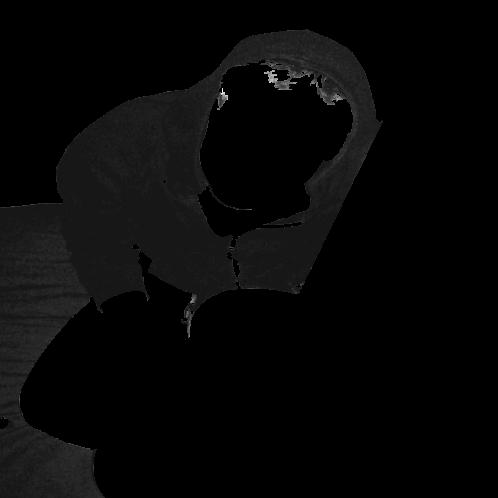
\includegraphics[width=\textwidth]{MSTseg4.jpg}
\end{minipage}
\caption{The original image is in the top left hand corner. The three largest segments are shown in the other corners. The original image was 498x498 and 50000 divisions were used.}
\label{mst:segmented}
\end{figure}
\vfill 
